\documentclass[tikz]{standalone}
\input{../tikz.tex.preamble}
\input{../typography.tex.preamble}

\begin{document}
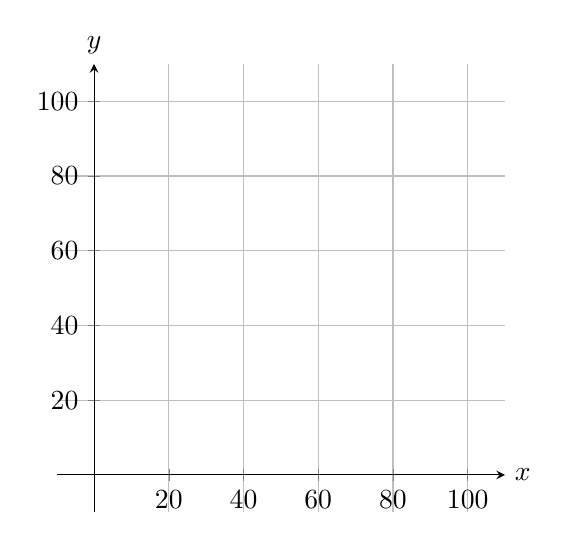
\begin{tikzpicture}
  \begin{axis}[
    axis equal image,
    axis lines=middle,
    enlargelimits=true,
    grid=both,
    scaled ticks=false,
    xmin=0, xmax=100,
    ymin=0, ymax=100,
    xlabel={\(x\)}, xlabel style={anchor=west},
    ylabel={\(y\)}, ylabel style={anchor=south},
    ]
  \end{axis}
\end{tikzpicture}

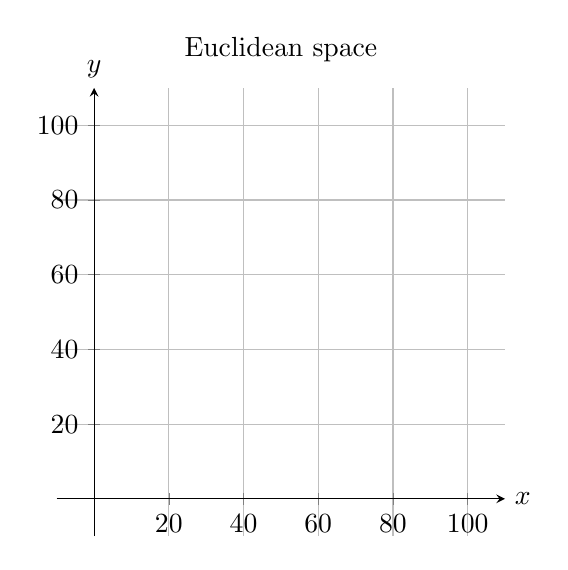
\begin{tikzpicture}
  \begin{axis}[
    axis equal image,
    axis lines=middle,
    enlargelimits=true,
    grid=both,
    scaled ticks=false,
    xmin=0, xmax=100,
    ymin=0, ymax=100,
    xlabel={\(x\)}, xlabel style={anchor=west},
    ylabel={\(y\)}, ylabel style={anchor=south},
    title={Euclidean space},
    ]
  \end{axis}
\end{tikzpicture}

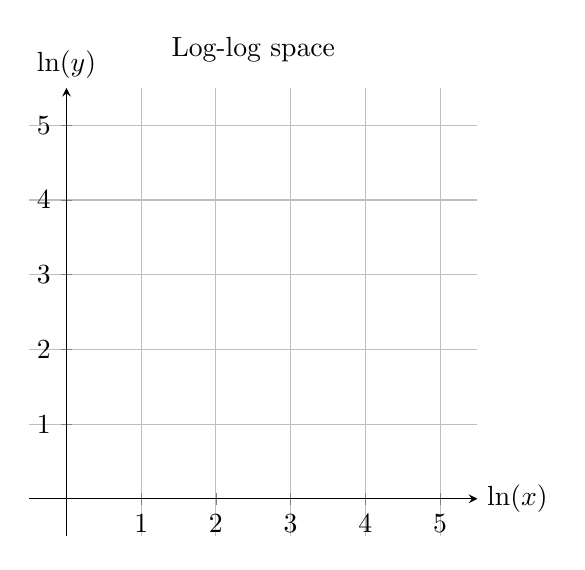
\begin{tikzpicture}
  \begin{axis}[
    axis equal image,
    axis lines=middle,
    enlargelimits=true,
    grid=both,
    scaled ticks=false,
    xtick={0,...,5},
    ytick={0,...,5},
    xmin=0, xmax=5,
    ymin=0, ymax=5,
    xlabel={\(\ln(x)\)}, xlabel style={anchor=west},
    ylabel={\(\ln(y)\)}, ylabel style={anchor=south},
    title={Log-log space},
    ]
  \end{axis}
\end{tikzpicture}
\end{document}
